


\tikzset{every picture/.style={line width=0.75pt}} %set default line width to 0.75pt        

\begin{tikzpicture}[x=0.75pt,y=0.75pt,yscale=-1,xscale=1]
%uncomment if require: \path (0,4289); %set diagram left start at 0, and has height of 4289

%Straight Lines [id:da7946343896752899] 
\draw [color={rgb, 255:red, 74; green, 144; blue, 226 }  ,draw opacity=1 ][line width=2.25]    (321.31,3515.13) -- (364.17,3515.13) ;
\draw [shift={(369.17,3515.13)}, rotate = 180] [fill={rgb, 255:red, 74; green, 144; blue, 226 }  ,fill opacity=1 ][line width=0.08]  [draw opacity=0] (5.72,-2.75) -- (0,0) -- (5.72,2.75) -- cycle    ;
%Image [id:dp21978411358424443] 
\draw (113.77,3463.95) node  {
\includegraphics[width=18.66pt,height=18.36pt]{figures/karma_architecture/pod.png}};
%Image [id:dp9349311722784455] 
\draw (152.86,3463.95) node  {
\includegraphics[width=18.66pt,height=18.36pt]{figures/karma_architecture/pod.png}};
%Shape: Rectangle [id:dp23088311220487756] 
\draw  [color={rgb, 255:red, 74; green, 144; blue, 226 }  ,draw opacity=1 ][line width=1.5]  (96,3431.36) .. controls (96,3428.6) and (98.24,3426.36) .. (101,3426.36) -- (253.68,3426.36) .. controls (256.44,3426.36) and (258.68,3428.6) .. (258.68,3431.36) -- (258.68,3535) .. controls (258.68,3537.76) and (256.44,3540) .. (253.68,3540) -- (101,3540) .. controls (98.24,3540) and (96,3537.76) .. (96,3535) -- cycle ;
%Image [id:dp858362205299811] 
\draw (172.41,3420.24) node  {
\includegraphics[width=18.66pt,height=18.36pt]{figures/karma_architecture/kubernetes.png}};
%Image [id:dp46926588962236737] 
\draw (231.67,3474.02) node  {
\includegraphics[width=18.66pt,height=18.36pt]{figures/karma_architecture/api.png}};
%Shape: Rectangle [id:dp32375406543307217] 
\draw  [color={rgb, 255:red, 255; green, 255; blue, 255 }  ,draw opacity=1 ][fill={rgb, 255:red, 255; green, 255; blue, 255 }  ,fill opacity=1 ] (220.39,3513.77) -- (241.72,3513.77) -- (241.72,3519.02) -- (220.39,3519.02) -- cycle ;
%Image [id:dp42326382110210514] 
\draw (231.05,3515.5) node  {
\includegraphics[width=18.66pt,height=18.36pt]{figures/karma_architecture/prometheus.png}};
%Shape: Rectangle [id:dp2965561697811463] 
\draw  [color={rgb, 255:red, 74; green, 144; blue, 226 }  ,draw opacity=1 ][line width=1.5]  (99.55,3453.21) .. controls (99.55,3450.45) and (101.79,3448.21) .. (104.55,3448.21) -- (162.08,3448.21) .. controls (164.84,3448.21) and (167.08,3450.45) .. (167.08,3453.21) -- (167.08,3473.81) .. controls (167.08,3476.57) and (164.84,3478.81) .. (162.08,3478.81) -- (104.55,3478.81) .. controls (101.79,3478.81) and (99.55,3476.57) .. (99.55,3473.81) -- cycle ;
%Image [id:dp02408756390394662] 
\draw (133.32,3442.97) node  {
\includegraphics[width=18.66pt,height=18.36pt]{figures/karma_architecture/node.png}};
%Image [id:dp2610546420725961] 
\draw (113.77,3522.52) node  {
\includegraphics[width=18.66pt,height=18.36pt]{figures/karma_architecture/pod.png}};
%Image [id:dp4744764852976593] 
\draw (152.86,3522.52) node  {
\includegraphics[width=18.66pt,height=18.36pt]{figures/karma_architecture/pod.png}};
%Shape: Rectangle [id:dp09571804252453764] 
\draw  [color={rgb, 255:red, 74; green, 144; blue, 226 }  ,draw opacity=1 ][line width=1.5]  (99.55,3511.78) .. controls (99.55,3509.02) and (101.79,3506.78) .. (104.55,3506.78) -- (162.08,3506.78) .. controls (164.84,3506.78) and (167.08,3509.02) .. (167.08,3511.78) -- (167.08,3532.38) .. controls (167.08,3535.14) and (164.84,3537.38) .. (162.08,3537.38) -- (104.55,3537.38) .. controls (101.79,3537.38) and (99.55,3535.14) .. (99.55,3532.38) -- cycle ;
%Image [id:dp38237667087549276] 
\draw (133.32,3501.54) node  {
\includegraphics[width=18.66pt,height=18.36pt]{figures/karma_architecture/node.png}};
%Shape: Rectangle [id:dp3796351069112436] 
\draw  [color={rgb, 255:red, 74; green, 144; blue, 226 }  ,draw opacity=1 ][line width=1.5]  (263.04,3431.36) .. controls (263.04,3428.6) and (265.28,3426.36) .. (268.04,3426.36) -- (418.78,3426.36) .. controls (421.54,3426.36) and (423.78,3428.6) .. (423.78,3431.36) -- (423.78,3535) .. controls (423.78,3537.76) and (421.54,3540) .. (418.78,3540) -- (268.04,3540) .. controls (265.28,3540) and (263.04,3537.76) .. (263.04,3535) -- cycle ;
%Image [id:dp7477281986060205] 
\draw (193.74,3494.54) node  {
\includegraphics[width=18.66pt,height=18.36pt]{figures/karma_architecture/deploy.png}};
%Straight Lines [id:da5822161786648565] 
\draw [color={rgb, 255:red, 74; green, 144; blue, 226 }  ,draw opacity=1 ][line width=2.25]    (170.63,3515.5) -- (211.84,3515.5) ;
\draw [shift={(216.84,3515.5)}, rotate = 180] [fill={rgb, 255:red, 74; green, 144; blue, 226 }  ,fill opacity=1 ][line width=0.08]  [draw opacity=0] (5.72,-2.75) -- (0,0) -- (5.72,2.75) -- cycle    ;
%Straight Lines [id:da6752650173025212] 
\draw [color={rgb, 255:red, 74; green, 144; blue, 226 }  ,draw opacity=1 ][line width=2.25]    (181.3,3496.29) -- (173.86,3496.29) ;
\draw [shift={(168.86,3496.29)}, rotate = 360] [fill={rgb, 255:red, 74; green, 144; blue, 226 }  ,fill opacity=1 ][line width=0.08]  [draw opacity=0] (5.72,-2.75) -- (0,0) -- (5.72,2.75) -- cycle    ;
%Straight Lines [id:da5574521680373876] 
\draw [color={rgb, 255:red, 74; green, 144; blue, 226 }  ,draw opacity=1 ][line width=2.25]    (217.4,3476.44) -- (210.26,3476.44) ;
\draw [shift={(205.26,3476.44)}, rotate = 360] [fill={rgb, 255:red, 74; green, 144; blue, 226 }  ,fill opacity=1 ][line width=0.08]  [draw opacity=0] (5.72,-2.75) -- (0,0) -- (5.72,2.75) -- cycle    ;
%Image [id:dp2482885261502139] 
\draw (193.74,3461.32) node  {
\includegraphics[width=18.66pt,height=18.36pt]{figures/karma_architecture/deploy.png}};
%Straight Lines [id:da48196313267418356] 
\draw [color={rgb, 255:red, 74; green, 144; blue, 226 }  ,draw opacity=1 ][line width=2.25]    (181.3,3463.07) -- (173.86,3463.07) ;
\draw [shift={(168.86,3463.07)}, rotate = 360] [fill={rgb, 255:red, 74; green, 144; blue, 226 }  ,fill opacity=1 ][line width=0.08]  [draw opacity=0] (5.72,-2.75) -- (0,0) -- (5.72,2.75) -- cycle    ;
%Straight Lines [id:da019658715417344652] 
\draw [color={rgb, 255:red, 74; green, 144; blue, 226 }  ,draw opacity=1 ][line width=2.25]    (273.46,3476.28) -- (248.55,3476.28) ;
\draw [shift={(243.55,3476.28)}, rotate = 360] [fill={rgb, 255:red, 74; green, 144; blue, 226 }  ,fill opacity=1 ][line width=0.08]  [draw opacity=0] (5.72,-2.75) -- (0,0) -- (5.72,2.75) -- cycle    ;
%Straight Lines [id:da0770687376267245] 
\draw [color={rgb, 255:red, 74; green, 144; blue, 226 }  ,draw opacity=1 ][line width=2.25]    (268.76,3514.51) -- (248.55,3514.51) ;
\draw [shift={(243.55,3514.51)}, rotate = 360] [fill={rgb, 255:red, 74; green, 144; blue, 226 }  ,fill opacity=1 ][line width=0.08]  [draw opacity=0] (5.72,-2.75) -- (0,0) -- (5.72,2.75) -- cycle    ;
\draw [shift={(273.76,3514.51)}, rotate = 180] [fill={rgb, 255:red, 74; green, 144; blue, 226 }  ,fill opacity=1 ][line width=0.08]  [draw opacity=0] (5.72,-2.75) -- (0,0) -- (5.72,2.75) -- cycle    ;
%Shape: Rectangle [id:dp6175004880171007] 
\draw  [color={rgb, 255:red, 255; green, 255; blue, 255 }  ,draw opacity=1 ][fill={rgb, 255:red, 255; green, 255; blue, 255 }  ,fill opacity=1 ] (332.92,3510.67) -- (357.2,3510.67) -- (357.2,3518) -- (332.92,3518) -- cycle ;
%Image [id:dp10400421500894241] 
\draw (345.77,3513.47) node  {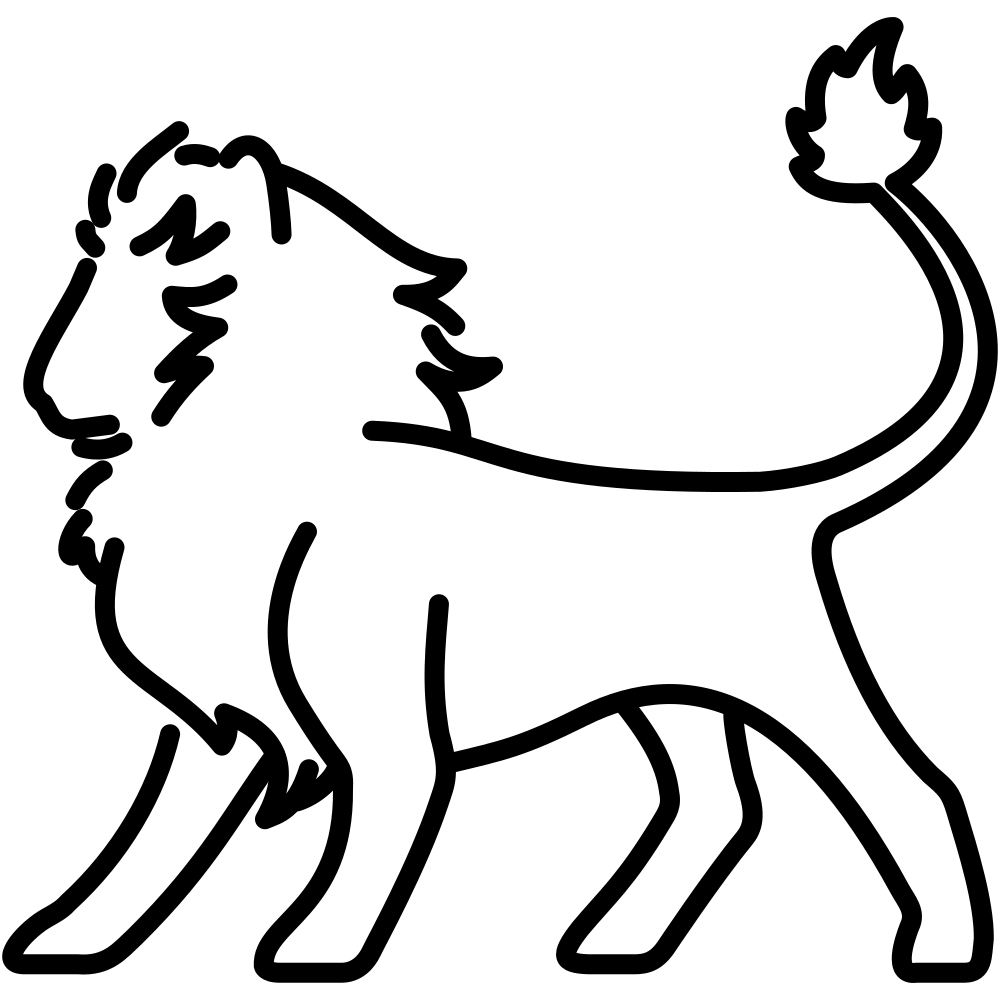
\includegraphics[width=14.57pt,height=15.21pt]{figures/karma_architecture/pettingzoo.png}};
%Straight Lines [id:da5805977657851873] 
\draw [color={rgb, 255:red, 74; green, 144; blue, 226 }  ,draw opacity=1 ][line width=2.25]    (364.2,3445.32) -- (369.17,3445.32) ;
\draw [shift={(359.2,3445.32)}, rotate = 0] [fill={rgb, 255:red, 74; green, 144; blue, 226 }  ,fill opacity=1 ][line width=0.08]  [draw opacity=0] (5.72,-2.75) -- (0,0) -- (5.72,2.75) -- cycle    ;
%Straight Lines [id:da08245916437277212] 
\draw [color={rgb, 255:red, 74; green, 144; blue, 226 }  ,draw opacity=1 ][line width=2.25]    (395.09,3501.77) -- (395.09,3461.25) ;
\draw [shift={(395.09,3456.25)}, rotate = 90] [fill={rgb, 255:red, 74; green, 144; blue, 226 }  ,fill opacity=1 ][line width=0.08]  [draw opacity=0] (5.72,-2.75) -- (0,0) -- (5.72,2.75) -- cycle    ;
%Straight Lines [id:da9595066849660663] 
\draw [color={rgb, 255:red, 74; green, 144; blue, 226 }  ,draw opacity=1 ][line width=2.25]    (397.07,3476.44) -- (328.31,3476.29) ;
\draw [shift={(323.31,3476.28)}, rotate = 0.13] [fill={rgb, 255:red, 74; green, 144; blue, 226 }  ,fill opacity=1 ][line width=0.08]  [draw opacity=0] (5.72,-2.75) -- (0,0) -- (5.72,2.75) -- cycle    ;
%Shape: Rectangle [id:dp02233992750973668] 
\draw  [color={rgb, 255:red, 255; green, 255; blue, 255 }  ,draw opacity=1 ][fill={rgb, 255:red, 255; green, 255; blue, 255 }  ,fill opacity=1 ] (382.51,3469.11) -- (401.93,3469.11) -- (401.93,3496) -- (382.51,3496) -- cycle ;
%Shape: Smiley Face [id:dp11323105399588185] 
\draw  [fill={rgb, 255:red, 255; green, 255; blue, 255 }  ,fill opacity=1 ][line width=0.75]  (384.45,3473.4) .. controls (384.45,3471.3) and (386.19,3469.6) .. (388.33,3469.6) .. controls (390.48,3469.6) and (392.22,3471.3) .. (392.22,3473.4) .. controls (392.22,3475.5) and (390.48,3477.2) .. (388.33,3477.2) .. controls (386.19,3477.2) and (384.45,3475.5) .. (384.45,3473.4) -- cycle ; \draw  [fill={rgb, 255:red, 255; green, 255; blue, 255 }  ,fill opacity=1 ][line width=0.75]  (386.62,3472.11) .. controls (386.62,3471.9) and (386.8,3471.73) .. (387.01,3471.73) .. controls (387.23,3471.73) and (387.4,3471.9) .. (387.4,3472.11) .. controls (387.4,3472.32) and (387.23,3472.49) .. (387.01,3472.49) .. controls (386.8,3472.49) and (386.62,3472.32) .. (386.62,3472.11) -- cycle ; \draw  [fill={rgb, 255:red, 255; green, 255; blue, 255 }  ,fill opacity=1 ][line width=0.75]  (389.27,3472.11) .. controls (389.27,3471.9) and (389.44,3471.73) .. (389.65,3471.73) .. controls (389.87,3471.73) and (390.04,3471.9) .. (390.04,3472.11) .. controls (390.04,3472.32) and (389.87,3472.49) .. (389.65,3472.49) .. controls (389.44,3472.49) and (389.27,3472.32) .. (389.27,3472.11) -- cycle ; \draw  [line width=0.75]  (386.39,3474.92) .. controls (387.69,3475.94) and (388.98,3475.94) .. (390.28,3474.92) ;
%Shape: Smiley Face [id:dp5398162097950316] 
\draw  [fill={rgb, 255:red, 255; green, 255; blue, 255 }  ,fill opacity=1 ][line width=0.75]  (396.1,3473.4) .. controls (396.1,3471.3) and (397.84,3469.6) .. (399.99,3469.6) .. controls (402.13,3469.6) and (403.87,3471.3) .. (403.87,3473.4) .. controls (403.87,3475.5) and (402.13,3477.2) .. (399.99,3477.2) .. controls (397.84,3477.2) and (396.1,3475.5) .. (396.1,3473.4) -- cycle ; \draw  [fill={rgb, 255:red, 255; green, 255; blue, 255 }  ,fill opacity=1 ][line width=0.75]  (398.28,3472.11) .. controls (398.28,3471.9) and (398.45,3471.73) .. (398.67,3471.73) .. controls (398.88,3471.73) and (399.05,3471.9) .. (399.05,3472.11) .. controls (399.05,3472.32) and (398.88,3472.49) .. (398.67,3472.49) .. controls (398.45,3472.49) and (398.28,3472.32) .. (398.28,3472.11) -- cycle ; \draw  [fill={rgb, 255:red, 255; green, 255; blue, 255 }  ,fill opacity=1 ][line width=0.75]  (400.92,3472.11) .. controls (400.92,3471.9) and (401.09,3471.73) .. (401.31,3471.73) .. controls (401.52,3471.73) and (401.7,3471.9) .. (401.7,3472.11) .. controls (401.7,3472.32) and (401.52,3472.49) .. (401.31,3472.49) .. controls (401.09,3472.49) and (400.92,3472.32) .. (400.92,3472.11) -- cycle ; \draw  [line width=0.75]  (398.04,3474.92) .. controls (399.34,3475.94) and (400.63,3475.94) .. (401.93,3474.92) ;
%Shape: Smiley Face [id:dp7737647671472778] 
\draw  [fill={rgb, 255:red, 255; green, 255; blue, 255 }  ,fill opacity=1 ][line width=0.75]  (390.28,3481.44) .. controls (390.28,3479.34) and (392.01,3477.64) .. (394.16,3477.64) .. controls (396.31,3477.64) and (398.04,3479.34) .. (398.04,3481.44) .. controls (398.04,3483.54) and (396.31,3485.24) .. (394.16,3485.24) .. controls (392.01,3485.24) and (390.28,3483.54) .. (390.28,3481.44) -- cycle ; \draw  [fill={rgb, 255:red, 255; green, 255; blue, 255 }  ,fill opacity=1 ][line width=0.75]  (392.45,3480.15) .. controls (392.45,3479.94) and (392.62,3479.77) .. (392.84,3479.77) .. controls (393.05,3479.77) and (393.23,3479.94) .. (393.23,3480.15) .. controls (393.23,3480.36) and (393.05,3480.53) .. (392.84,3480.53) .. controls (392.62,3480.53) and (392.45,3480.36) .. (392.45,3480.15) -- cycle ; \draw  [fill={rgb, 255:red, 255; green, 255; blue, 255 }  ,fill opacity=1 ][line width=0.75]  (395.09,3480.15) .. controls (395.09,3479.94) and (395.27,3479.77) .. (395.48,3479.77) .. controls (395.7,3479.77) and (395.87,3479.94) .. (395.87,3480.15) .. controls (395.87,3480.36) and (395.7,3480.53) .. (395.48,3480.53) .. controls (395.27,3480.53) and (395.09,3480.36) .. (395.09,3480.15) -- cycle ; \draw  [line width=0.75]  (392.22,3482.96) .. controls (393.51,3483.98) and (394.81,3483.98) .. (396.1,3482.96) ;
%Flowchart: Punched Tape [id:dp9180210416243069] 
\draw  [fill={rgb, 255:red, 255; green, 255; blue, 255 }  ,fill opacity=1 ] (319.32,3437.81) .. controls (319.32,3439.03) and (323.78,3440.02) .. (329.29,3440.02) .. controls (334.79,3440.02) and (339.26,3439.03) .. (339.26,3437.81) .. controls (339.26,3436.58) and (343.72,3435.59) .. (349.23,3435.59) .. controls (354.73,3435.59) and (359.2,3436.58) .. (359.2,3437.81) -- (359.2,3455.52) .. controls (359.2,3454.3) and (354.73,3453.31) .. (349.23,3453.31) .. controls (343.72,3453.31) and (339.26,3454.3) .. (339.26,3455.52) .. controls (339.26,3456.75) and (334.79,3457.74) .. (329.29,3457.74) .. controls (323.78,3457.74) and (319.32,3456.75) .. (319.32,3455.52) -- cycle ;
%Straight Lines [id:da6274111550180377] 
\draw [line width=1.5]    (332.07,3444.17) -- (346.86,3442.47) ;
\draw [shift={(349.84,3442.13)}, rotate = 173.45] [color={rgb, 255:red, 0; green, 0; blue, 0 }  ][line width=1.5]    (5.68,-1.71) .. controls (3.61,-0.72) and (1.72,-0.15) .. (0,0) .. controls (1.72,0.15) and (3.61,0.72) .. (5.68,1.71)   ;
%Shape: Smiley Face [id:dp08006052667693364] 
\draw  [line width=0.75]  (327.67,3444.88) .. controls (327.67,3443.7) and (328.69,3442.73) .. (329.94,3442.73) .. controls (331.19,3442.73) and (332.21,3443.7) .. (332.21,3444.88) .. controls (332.21,3446.07) and (331.19,3447.03) .. (329.94,3447.03) .. controls (328.69,3447.03) and (327.67,3446.07) .. (327.67,3444.88) -- cycle ; \draw  [line width=0.75]  (328.94,3444.15) .. controls (328.94,3444.03) and (329.05,3443.94) .. (329.17,3443.94) .. controls (329.3,3443.94) and (329.4,3444.03) .. (329.4,3444.15) .. controls (329.4,3444.27) and (329.3,3444.37) .. (329.17,3444.37) .. controls (329.05,3444.37) and (328.94,3444.27) .. (328.94,3444.15) -- cycle ; \draw  [line width=0.75]  (330.49,3444.15) .. controls (330.49,3444.03) and (330.59,3443.94) .. (330.71,3443.94) .. controls (330.84,3443.94) and (330.94,3444.03) .. (330.94,3444.15) .. controls (330.94,3444.27) and (330.84,3444.37) .. (330.71,3444.37) .. controls (330.59,3444.37) and (330.49,3444.27) .. (330.49,3444.15) -- cycle ; \draw  [line width=0.75]  (328.81,3445.74) .. controls (329.56,3446.31) and (330.32,3446.31) .. (331.07,3445.74) ;
%Shape: Smiley Face [id:dp015117611383586027] 
\draw  [line width=0.75]  (342.18,3450.61) .. controls (342.18,3449.42) and (343.2,3448.46) .. (344.45,3448.46) .. controls (345.7,3448.46) and (346.71,3449.42) .. (346.71,3450.61) .. controls (346.71,3451.79) and (345.7,3452.76) .. (344.45,3452.76) .. controls (343.2,3452.76) and (342.18,3451.79) .. (342.18,3450.61) -- cycle ; \draw  [line width=0.75]  (343.45,3449.88) .. controls (343.45,3449.76) and (343.55,3449.66) .. (343.68,3449.66) .. controls (343.8,3449.66) and (343.9,3449.76) .. (343.9,3449.88) .. controls (343.9,3450) and (343.8,3450.09) .. (343.68,3450.09) .. controls (343.55,3450.09) and (343.45,3450) .. (343.45,3449.88) -- cycle ; \draw  [line width=0.75]  (344.99,3449.88) .. controls (344.99,3449.76) and (345.09,3449.66) .. (345.22,3449.66) .. controls (345.34,3449.66) and (345.45,3449.76) .. (345.45,3449.88) .. controls (345.45,3450) and (345.34,3450.09) .. (345.22,3450.09) .. controls (345.09,3450.09) and (344.99,3450) .. (344.99,3449.88) -- cycle ; \draw  [line width=0.75]  (343.31,3451.47) .. controls (344.07,3452.04) and (344.83,3452.04) .. (345.58,3451.47) ;
%Shape: Smiley Face [id:dp09027993713421267] 
\draw  [line width=0.75]  (350.3,3442.59) .. controls (350.3,3441.4) and (351.32,3440.44) .. (352.57,3440.44) .. controls (353.82,3440.44) and (354.84,3441.4) .. (354.84,3442.59) .. controls (354.84,3443.78) and (353.82,3444.74) .. (352.57,3444.74) .. controls (351.32,3444.74) and (350.3,3443.78) .. (350.3,3442.59) -- cycle ; \draw  [line width=0.75]  (351.57,3441.86) .. controls (351.57,3441.74) and (351.68,3441.65) .. (351.8,3441.65) .. controls (351.93,3441.65) and (352.03,3441.74) .. (352.03,3441.86) .. controls (352.03,3441.98) and (351.93,3442.08) .. (351.8,3442.08) .. controls (351.68,3442.08) and (351.57,3441.98) .. (351.57,3441.86) -- cycle ; \draw  [line width=0.75]  (353.12,3441.86) .. controls (353.12,3441.74) and (353.22,3441.65) .. (353.34,3441.65) .. controls (353.47,3441.65) and (353.57,3441.74) .. (353.57,3441.86) .. controls (353.57,3441.98) and (353.47,3442.08) .. (353.34,3442.08) .. controls (353.22,3442.08) and (353.12,3441.98) .. (353.12,3441.86) -- cycle ; \draw  [line width=0.75]  (351.44,3443.45) .. controls (352.19,3444.02) and (352.95,3444.02) .. (353.7,3443.45) ;
%Straight Lines [id:da3860464645873938] 
\draw [line width=1.5]    (331.28,3445.87) -- (338.62,3449.89) ;
\draw [shift={(341.25,3451.33)}, rotate = 208.72] [color={rgb, 255:red, 0; green, 0; blue, 0 }  ][line width=1.5]    (5.68,-1.71) .. controls (3.61,-0.72) and (1.72,-0.15) .. (0,0) .. controls (1.72,0.15) and (3.61,0.72) .. (5.68,1.71)   ;



% Text Node
\draw  [color={rgb, 255:red, 75; green, 101; blue, 225 }  ,draw opacity=1 ][fill={rgb, 255:red, 136; green, 197; blue, 246 }  ,fill opacity=1 ][line width=1.5]   (329.27,3417.89) .. controls (329.27,3416.78) and (330.17,3415.89) .. (331.27,3415.89) -- (363.27,3415.89) .. controls (364.38,3415.89) and (365.27,3416.78) .. (365.27,3417.89) -- (365.27,3429.89) .. controls (365.27,3430.99) and (364.38,3431.89) .. (363.27,3431.89) -- (331.27,3431.89) .. controls (330.17,3431.89) and (329.27,3430.99) .. (329.27,3429.89) -- cycle  ;
\draw (347.27,3423.89) node  [font=\tiny] [align=left] {\begin{minipage}[lt]{21.5pt}\setlength\topsep{0pt}
\begin{center}
KARMA
\end{center}

\end{minipage}};
% Text Node
\draw (294.42,3445.42) node  [font=\tiny] [align=left] {\begin{minipage}[lt]{27.24pt}\setlength\topsep{0pt}
\begin{center}
Organizational\\Analysis
\end{center}

\end{minipage}};
% Text Node
\draw (392.1,3490.39) node  [font=\tiny] [align=left] {\begin{minipage}[lt]{43.42pt}\setlength\topsep{0pt}
\begin{center}
Trained policies
\end{center}

\end{minipage}};
% Text Node
\draw (348.23,3531.35) node  [font=\tiny] [align=left] {\begin{minipage}[lt]{60.78pt}\setlength\topsep{0pt}
\begin{center}
PettingZoo environment
\end{center}

\end{minipage}};
% Text Node
\draw (225.45,3531.39) node  [font=\tiny] [align=left] {\begin{minipage}[lt]{23.15pt}\setlength\topsep{0pt}
\begin{center}
Prometheus
\end{center}

\end{minipage}};
% Text Node
\draw  [color={rgb, 255:red, 75; green, 101; blue, 225 }  ,draw opacity=1 ][fill={rgb, 255:red, 136; green, 197; blue, 246 }  ,fill opacity=1 ][line width=1.5]   (274.27,3465.32) .. controls (274.27,3464.22) and (275.17,3463.32) .. (276.27,3463.32) -- (319.27,3463.32) .. controls (320.37,3463.32) and (321.27,3464.22) .. (321.27,3465.32) -- (321.27,3486.32) .. controls (321.27,3487.43) and (320.37,3488.32) .. (319.27,3488.32) -- (276.27,3488.32) .. controls (275.17,3488.32) and (274.27,3487.43) .. (274.27,3486.32) -- cycle  ;
\draw (297.77,3475.82) node  [font=\tiny,color={rgb, 255:red, 0; green, 0; blue, 0 }  ,opacity=1 ] [align=left] {Transfer\\Component};
% Text Node
\draw  [color={rgb, 255:red, 75; green, 101; blue, 225 }  ,draw opacity=1 ][fill={rgb, 255:red, 136; green, 197; blue, 246 }  ,fill opacity=1 ][line width=1.5]   (369.98,3433.46) .. controls (369.98,3432.35) and (370.87,3431.46) .. (371.98,3431.46) -- (414.98,3431.46) .. controls (416.08,3431.46) and (416.98,3432.35) .. (416.98,3433.46) -- (416.98,3454.46) .. controls (416.98,3455.56) and (416.08,3456.46) .. (414.98,3456.46) -- (371.98,3456.46) .. controls (370.87,3456.46) and (369.98,3455.56) .. (369.98,3454.46) -- cycle  ;
\draw (393.48,3443.96) node  [font=\tiny,color={rgb, 255:red, 0; green, 0; blue, 0 }  ,opacity=1 ] [align=left] {Analyzing\\Component};
% Text Node
\draw  [color={rgb, 255:red, 75; green, 101; blue, 225 }  ,draw opacity=1 ][fill={rgb, 255:red, 136; green, 197; blue, 246 }  ,fill opacity=1 ][line width=1.5]   (369.98,3502.24) .. controls (369.98,3501.13) and (370.87,3500.24) .. (371.98,3500.24) -- (414.98,3500.24) .. controls (416.08,3500.24) and (416.98,3501.13) .. (416.98,3502.24) -- (416.98,3523.24) .. controls (416.98,3524.34) and (416.08,3525.24) .. (414.98,3525.24) -- (371.98,3525.24) .. controls (370.87,3525.24) and (369.98,3524.34) .. (369.98,3523.24) -- cycle  ;
\draw (393.48,3512.74) node  [font=\tiny,color={rgb, 255:red, 0; green, 0; blue, 0 }  ,opacity=1 ] [align=left] {Training\\Component};
% Text Node
\draw (172.41,3437.36) node  [font=\tiny] [align=left] {\begin{minipage}[lt]{16.92pt}\setlength\topsep{0pt}
\begin{center}
Cluster
\end{center}

\end{minipage}};
% Text Node
\draw  [color={rgb, 255:red, 75; green, 101; blue, 225 }  ,draw opacity=1 ][fill={rgb, 255:red, 136; green, 197; blue, 246 }  ,fill opacity=1 ][line width=1.5]   (274.27,3502.64) .. controls (274.27,3501.54) and (275.17,3500.64) .. (276.27,3500.64) -- (319.27,3500.64) .. controls (320.37,3500.64) and (321.27,3501.54) .. (321.27,3502.64) -- (321.27,3523.64) .. controls (321.27,3524.75) and (320.37,3525.64) .. (319.27,3525.64) -- (276.27,3525.64) .. controls (275.17,3525.64) and (274.27,3524.75) .. (274.27,3523.64) -- cycle  ;
\draw (297.77,3513.14) node  [font=\tiny,color={rgb, 255:red, 0; green, 0; blue, 0 }  ,opacity=1 ] [align=left] {Modeling\\Component};
% Text Node
\draw (178.22,3478.11) node  [font=\tiny,rotate=-90] [align=left] {{\LARGE {\fontfamily{helvet}\selectfont \textcolor[rgb]{0.29,0.56,0.89}{...}}}};
% Text Node
\draw (132.61,3521.47) node  [font=\tiny] [align=left] {{\LARGE {\fontfamily{helvet}\selectfont \textcolor[rgb]{0.29,0.56,0.89}{...}}}};
% Text Node
\draw (155.16,3491.75) node  [font=\tiny,rotate=-90] [align=left] {{\LARGE {\fontfamily{helvet}\selectfont \textcolor[rgb]{0.29,0.56,0.89}{...}}}};
% Text Node
\draw (132.61,3462.9) node  [font=\tiny] [align=left] {{\LARGE {\fontfamily{helvet}\selectfont \textcolor[rgb]{0.29,0.56,0.89}{...}}}};
% Text Node
\draw (349.72,3436.31) node  [font=\tiny] [align=left] {\begin{minipage}[lt]{8.67pt}\setlength\topsep{0pt}
\begin{center}
{\footnotesize $\displaystyle \mathbf{\textcolor[rgb]{0.82,0.01,0.11}{\pi }\textcolor[rgb]{0.82,0.01,0.11}{_{3}}}$}
\end{center}

\end{minipage}};
% Text Node
\draw (351.72,3447.24) node  [font=\tiny] [align=left] {\begin{minipage}[lt]{8.67pt}\setlength\topsep{0pt}
\begin{center}
{\footnotesize $\displaystyle \mathbf{\textcolor[rgb]{0.82,0.01,0.11}{\pi }\textcolor[rgb]{0.82,0.01,0.11}{_{2}}}$}
\end{center}

\end{minipage}};
% Text Node
\draw (325.8,3440.86) node  [font=\tiny] [align=left] {\begin{minipage}[lt]{8.67pt}\setlength\topsep{0pt}
\begin{center}
{\footnotesize $\displaystyle \mathbf{\textcolor[rgb]{0.82,0.01,0.11}{\pi }\textcolor[rgb]{0.82,0.01,0.11}{_{1}}}$}
\end{center}

\end{minipage}};


\end{tikzpicture}